\textbf{Решающие деревья.} 

\begin{figure}[H]
\centering
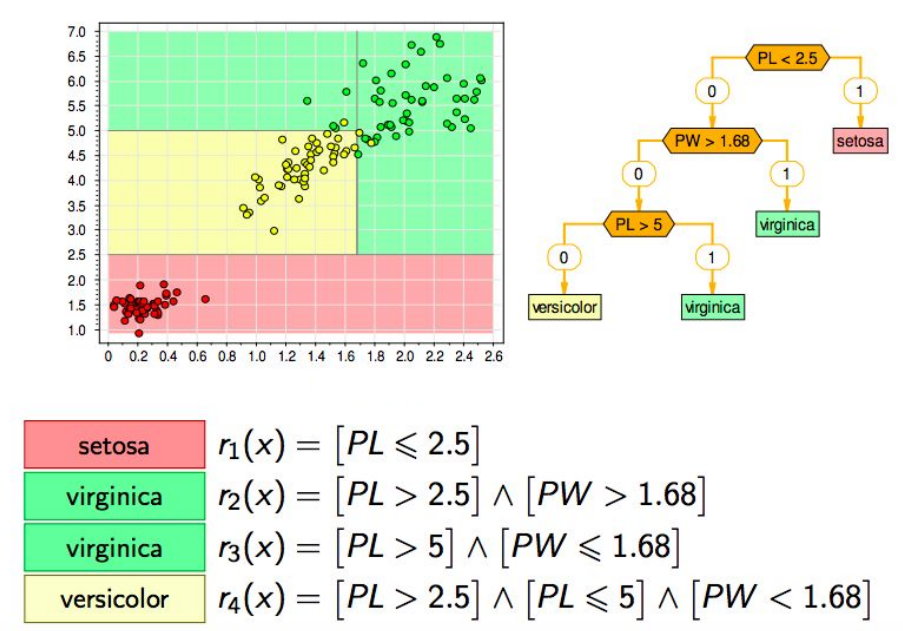
\includegraphics[width=0.5\linewidth]{16.1.PNG}
\caption{Датасет Ирисы Фишера и классификатор в виде дерева.}
\end{figure}

Поговорим об интуиции, лежащей под капотом решающего дерева. Давайте взглянем на знакомый датасет Ирисы Фишера. На рисунке ниже можем увидеть алгоритм классификации в виде дерева, который на каждом шаге использует предикат и с помощью этого делает какое-то решение одно из двух. Делаем на первом шаге разделение на два листа по значению 1го признака. В первый класс попали все объекты класса setosa, в нулевой класс всё остальное. Теперь по значению второго признаку, мы делим оставшуюся часть пространства пополам. Всё, что попало в класс 1 - virginica, в класс 0 остались зелёные и жёлтые признаки. Следующий шаг опять в делении по уже другому трешхолду 1го признака на две выборки, в одной из них virginica, в другой желтый versicolor. На рисунке дерево глубины 3, но некоторые объекты проклассифицировались неправильно,
поэтому мы можем достроить дерево более глубоким, чтобы все точки были проклассифицированы правильно. С одной стороны было бы хорошо так точно угадывать класс, но с другой стороны мы получим очень глубокое, то есть переобученное дерево. Так как мы пытаемся уловить возможно шумовые наблюдения в нашей обучающей выборке, мы переобучаемся под неё и теряем общую идею, которую мы могли бы перенести в тестовую выборку. Если присмотреться к такому классификатору, можно заметить, что каждому подпространству модель предсказывает константу. Если посмотреть на задачу регрессии на рисунке ниже, это видно ещё лучше. Тут изображён синус, который зашумлен и мы пытаемся описать эту гладкую функцию с помощью решающего дерева. В данном случае признаковое пространство 1мерное. Получается кусочно-постоянная функция. Потому что мы делим

\begin{figure}[h]
\centering
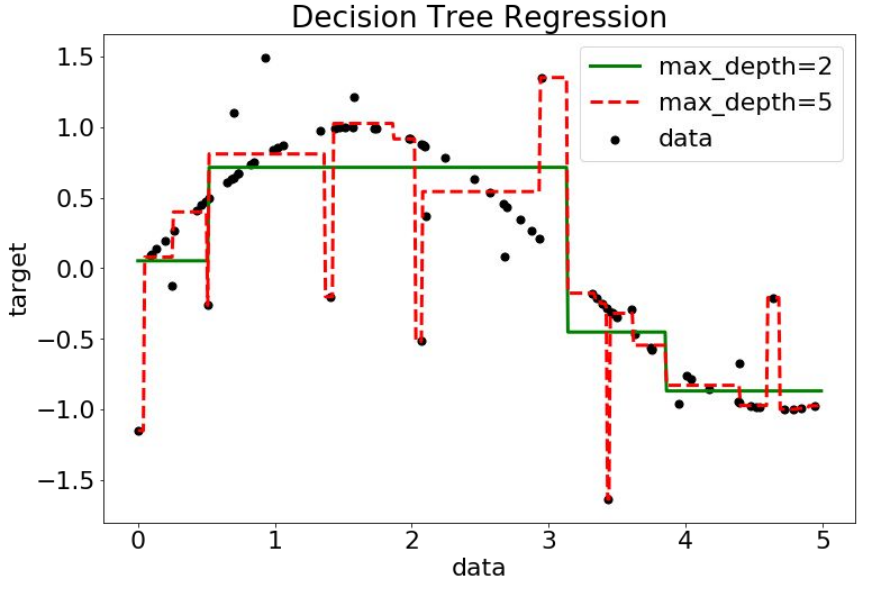
\includegraphics[width=0.5\linewidth]{16.2.PNG}
\caption{Решающие деревья в задаче регрессии.}
\end{figure}

признаковое пространство на куски и каждому куску сопоставляем некоторую константу. Красным показано дерево глубины 5, а зелёным - глубины 2. Мы видим, что красное дерево поймало шумовые точки - переобучилось. Так получилось, потому что на этих точках была большая ошибка, дерево пыталось минимизировать
ошибку и добилось такого фита. Дерево глубины 2 не очень хорошо описывает синус, но оно не переобучилось. Как нам построить дерево, а не просто применить построенное? Для этого нам требуется поставить оптимизационную задачу и обсудить как можно работать с деревом.

5.1 Построение модели решающего дерева

Сразу можно заметить, что поскольку функция, которую строит дерево кусочно-постоянная, а значит градиентные методы работать не будут (в каждом месте, где происходит разрыв, производная вообще не будет
определена). Нам придётся вернуться к жадной оптимизации за неимением лучшего метода.
\begin{enumerate}
    \item Пусть $x^{(j)}$ - $j$-ый признак
$$x^{(j)} < t$$

В данный момент времени мы находимся в ноде дерева, и в ней мы делим все объекты по j-ому признаку,
сравнивая его с трешхолдом t. Если признак у объекта меньше t, то объект идёт в левое поддерево, если
больше - в правое поддерево. Получаются две новые ноды (это левое и правое поддерево).
    \item  Делаем тоже самое для каждой новой ноды. Рекурсивный алгоритм.
\end{enumerate}


Откуда брать трешхолд и порог по индексу?

Поскольку датасает имеет конечное число признаков, которыми он описывается, то можно перебрать только конечное число трешхолдов, так как объектов тоже ограниченное количество. То есть будет 2 вложенных цикла: перебираем все возможные признаки, и все возможные трешхолды. 

Нам нужен формальный критерий, по которому мы можем понять насколько качественное разбиение. 

\begin{figure}[h]
\centering
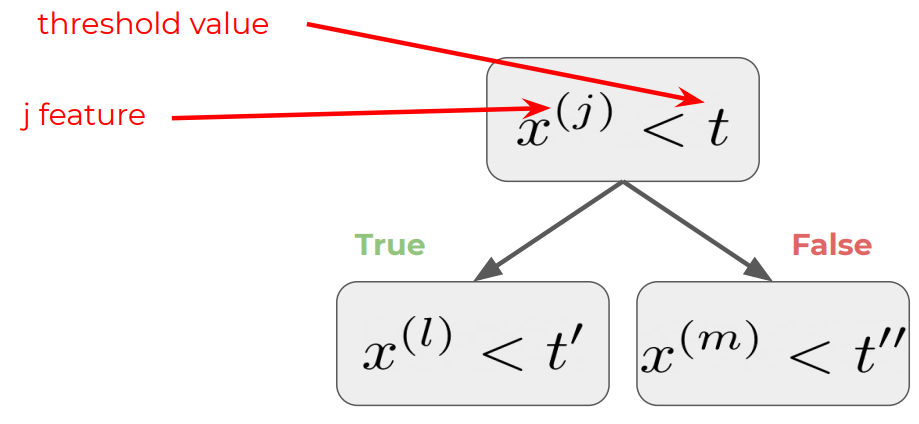
\includegraphics[width=0.5\linewidth]{16.3.PNG}
\caption{Иллюстрация разбиения в ноде.}
\end{figure} 

Пусть текущее условие $x^{(j)} < t$ действует в области $Q$. Условие  делит пространство $Q$ на две части $L$ и $R$. Введём функцию $G$ - взвешенную сумму функции информативности от левой, правой подвыборок:
$$G(j, t) = \frac{L}{Q} H(L) + \frac{R}{Q} H(R)$$
Логично, что в сумма $\frac{L}{Q} + \frac{R}{Q} = 1$.
$G(j, t)$ - указывает на то, насколько разбиение по $t$ является хорошим для нас. Чем значение больше, тем лучше.

Будем помнить, что дерево даёт только константу для каждого из листов (Это области, которые алгоритм не стал делить). Посмотрим на рисунок ниже. Для этого надо посчитать выборочные вероятности для классов встречающихся объектов в листе и выбрать наибольшую сумму.

\begin{figure}[h]
\centering
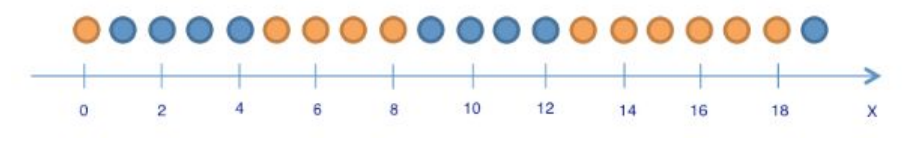
\includegraphics[width=0.5\linewidth]{16.4.PNG}
\caption{Классификация по 1 признаку.}
\end{figure}

Есть задание простое задание классифицировать шарики. Признак - одно число. И два класса.



Если нам надо разделить на 2 признака выборку по какой-то границе, то скорее всего мы обрежем так, чтобы с одной стороны доминировал один класс, а с другой - другой.

Обратите внимание на картинку ниже. Введём понятие упорядоченности или информационного критерия H(R). Под упорядоченностью понимается то, насколько сложно будет описать выборку, которая попала в лист. В простейшем случае бинарной классификации мы имеем дело с misclassification criteria:
$H(R) = 1 - max\{p_0, p_1\}$, где $p_0$ - доля значений класса 0 в выборке $R$, $p_1$ - доля класса 1 в выборке $R$. $p_0 + p_1 = 1$. 

\begin{figure}[h]
\centering
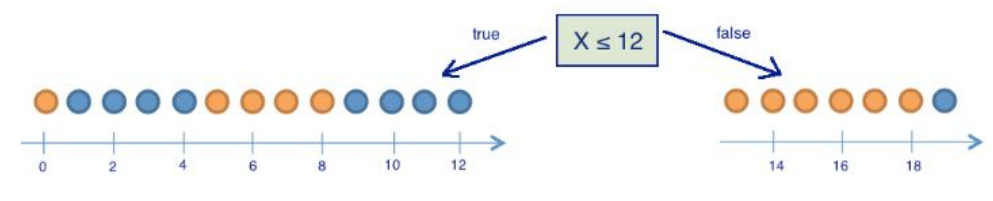
\includegraphics[width=0.5\linewidth]{16.5.PNG}
\caption{Разбиение на 2 подвыборки.}
\end{figure}

Оценивает 1 - выборочную вероятность данного класса. То есть по сути это вероятность ошибиться, если мы предсказываем самый доминирующий класс. Не очень хороший подход, потому что он игнорирует все недоминирующие классы, для многоклассовой классификации это плохо. Такой критерий приведен скорее для исторической справки. Нам важны следующие 2 критерия:
\begin{enumerate}
    \item  Entropy criteria:
$$H(R) = -p_0 \log p_0 - p_1 \log p_1 $$
    \item  Gini impurity:
$$H(R) = 1 - p_0^2 - p_1^2 = 1 - 2p_0p_1 $$
\end{enumerate}

Деревья, как и Наивный Байес работают с классификацией одинаково, вне зависимости от количества классов.